\subsection{Util}
Usualmente cometemos el error de intentar mantener al usuario lo mas informado posible y le ofrecemos datos que
no aportan informacion nueva, es redundate. Toda informacion vana, que no haga ninguna aportacion
al objetivo marcado tambien queda fuera de ser util.No queremos que el usuario se distraga o se pierda en medio
 de una piscina de datos completa pero compleja que para el no tenga ningun sentido. 

El objetivo no es crear usuarios especializados en la materia, sino aportarles la
informacion de una manera que la puedan aplicar a su vida diaria y asi mejorarla, mostrar datos
tecnicos, dificiles de interpretar solo hara que el usuario los evite

En caso complejos, los conceptos que no sean de uso diario para los usuario, podremos recurrir informacion
complementaria a su disposicion para que el usuario pueda informarse sobre el significado de los datos 
representados, esta practica proporcionara al usuario un mayor dominio del concepto y podra estar mas
seguro de su lectura de los datos, ya que cuando dirigimos al usuario a fuentes oficiales de informacion, donde puedan 
obtener una explicacion veridica,reenforzamos la credibilidad de las representaciones que estamos realizando. En todo caso, 
fuera de la representacion principal, porque el usuario no tendra que acceder a esta informacion continuamente.

\subsubsection{How to solve it} 
Centrarnos en el objetivo, mostrar los datos directamente relacionados con nuestra meta, no annadir los datos 
simplemente porque aparezcan en el conjunto de datos, y no annadir detalles tecnicos irrelevantes para el usuario.


\subsubsection{How we solve it. Aire Guru} 

El conjunto de datos utilizado contiene datos como el indicador de la estacion de medida, si la estacion es fija o movil
y medidas extra especificas para una aplicacion que proporciona la misma empresa que recoge los datos. Para nuestra
herramienta, estos datos no son utiles.
Para nuestra herramienta solo se han utilizado las coordenadas donde se encuentra la estacion de medicion, el momento en 
el que se realizo la medida y el valor mas relevante de los cinco contaminantes Co, No2, O3, Pm1, Pm 2.5 y Pm10.

Ademas, la medida es unica para todos y el general, el AQI, los rangos son exactamente los mismos para todos, asi el usuario
solo tiene que hacer el esfuerzo de enterder un unico concepto. 

Si la medida no existe, simplemente la obviaremos. No proporcionamos explicaciones o valores como 0 que pueden llegar a 
error, como si no existiera polucion.


En la figura siguiente vemos la diferencia entre el historial de zona y el personalizado, el primero de ellos no muestra
el punto donde se tomo la medida ya que se ha seleccionado en el mapa principal. Tambien emos como para el historial de 
zona no existe un filtro por horas, ya que las medidas son reportadas cada hora, esto significa que no encontraremos 
medidas intermedias en el conjunto de datos.
 
\begin{figure}[ht]
    \centering
    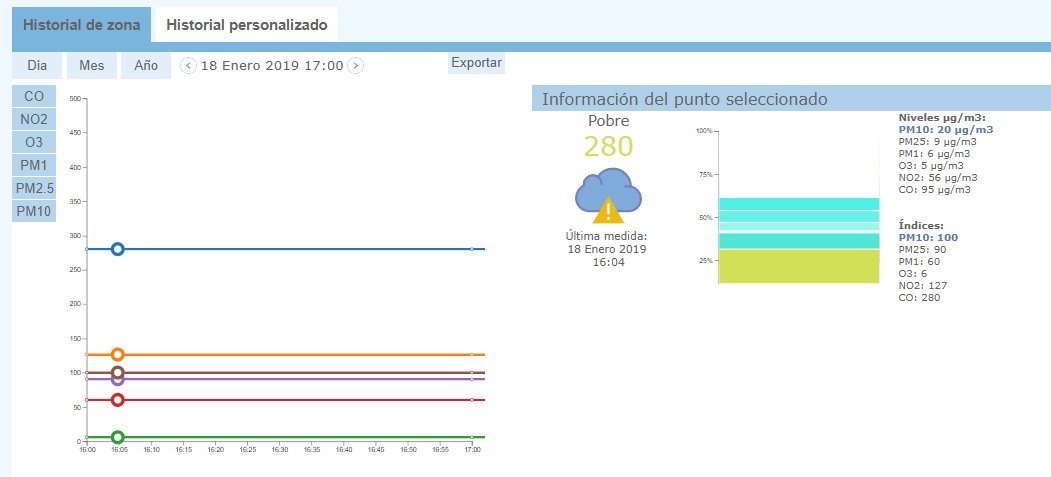
\includegraphics[width=11cm]{zoneRecords}
    \caption{Zone Records}
\end{figure}
\begin{figure}[ht]
    \centering
    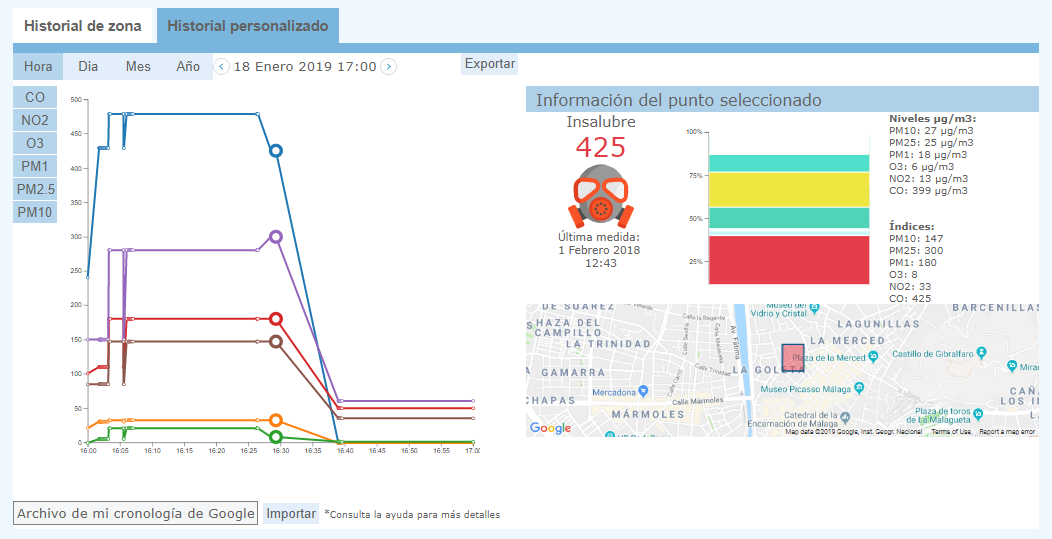
\includegraphics[width=11cm]{personalRecords}
    \caption{Personal Records}
\end{figure}


\elsparagraph{Evaluation}  
\begin{itemize}
    \done Se ha eliminado la informacion no relevante para el usuario.
    \crossed Se han ofrecido las mediciones exactas. Estos datos son demasiado tecnicos para el usuario. Sin embargo,
    aporta veracidad a los datos y se han  posicionado en un lugar secundario para que no distraiga al usuario.
    \crossed Se ha implementado una funcionalidad de exportar los datos, los comentarios de nuestros testers descubrieron
    que esta funcionalidad para el usuario medio no es util, ya que no cuentan con las herramientas necesarias para
    analizar los datos y toda la informacion esta en la herramienta representada en un mejor formato.
    
\end{itemize}
 \newpage